\section{Residues and descent across the conductor}\label{sec:residues}

The normal index theorem gives a uniformly bounded trivializing degree on
each component of the normalization.  The remaining question is whether
these trivializations can be chosen compatibly along the conductor.  We
will express each obstruction around a conductor cycle as the character
of a birational self-map of a single klt pair.  Theorem~\ref{thm:characters}
then kills every obstruction with the same exponent, independently of
the number of components and the length of the cycle.
This follows the established reduction from normal indices and bounded
pluricanonical representations to slc indices
\citep[Theorem~1.11]{Xu2019}.  We give the residue comparison explicitly,
using Koll\'ar's compatibility theorem inside each normalization component
and keeping the degree fixed throughout.

We first work over $\C$.  Throughout this section $m$ is a positive even
integer.  For a dlt pair $(Y,\Gamma)$, a \emph{stratum} means $Y$ itself
or an lc centre.  A minimal stratum is minimal for inclusion; thus it is
$Y$ if the pair is klt.  Dlt strata are normal, iterated adjunction gives
effective dlt pairs $(W,\Gamma_W)$ on them, and the strata of
$(W,\Gamma_W)$ are exactly the strata of $(Y,\Gamma)$ contained in $W$.
In particular, minimal strata are klt; see
\citep[Chapter~4]{Kollar2013} and \citep[Definition~4]{KollarSources}.

\subsection{Residues in a fixed degree}

Suppose that $(Y,\Gamma)$ is a projective integral dlt pair and that a
rational $m$-canonical form $\theta$ satisfies
\begin{equation}\label{res:form}
 \Div(\theta)=-m\Gamma.
\end{equation}
At the generic point of a codimension-$k$ stratum $W$, the pair is simple
normal crossing.  In local coordinates in which the coefficient-one
components through $W$ are $x_1\cdots x_k=0$, write
\[
 \theta=f\left(
 \frac{dx_1}{x_1}\wedge\cdots\wedge\frac{dx_k}{x_k}
 \wedge dy_1\wedge\cdots\wedge dy_{\dim W}
 \right)^{\otimes m}.
\]
Here $f$ is a unit at the generic point of $W$.  Its logarithmic residue
is the rational $m$-canonical form
\[
 \theta_W=f|_W\,(dy_1\wedge\cdots\wedge dy_{\dim W})^{\otimes m}.
\]
The usual residue transformation rule makes this definition independent
of the coordinates.  Reordering the normal coordinates changes an
ordinary residue by a sign, which disappears because $m$ is even.
Consequently residues along flags agree with direct iterated residues.
For $W=Y$, set $\theta_W=\theta$.

These forms satisfy the actual degree-$m$ identity
\begin{equation}\label{res:adjunction}
 \Div(\theta_W)=-m\Gamma_W,
 \qquad m(K_W+\Gamma_W)\sim0.
\end{equation}
Indeed, pluricanonical adjunction with the different gives this identity
for $\theta_W^{\otimes b}$ when $b$ is sufficiently divisible
\citep[Definition~13]{KollarSources}.  The generic residue construction
commutes with tensor powers, so division of that divisor identity by
$b$ gives \eqref{res:adjunction}.  In particular, $m\Gamma_W$ is integral.
No enlargement of $m$ depending on the stratum is required.

\begin{lemma}[Comparison within a dlt pair]\label{res:within}
 Let $(Y,\Gamma)$ and $\theta$ satisfy \eqref{res:form}.  For any two
 minimal strata $A,A'$, there is a B-birational map
 $\phi:(A,\Gamma_A)\dashrightarrow(A',\Gamma_{A'})$ such that
 \[
 \phi^*\theta_{A'}=\theta_A.
 \]
\end{lemma}

\begin{proof}
 There is nothing to prove if the pair is klt.  Otherwise apply
 \citet[Proposition~14]{KollarSources} to the morphism $Y\to\Spec\C$.
 Its hypotheses hold in degree $m$: the pair is dlt, its log canonical
 divisor is rationally trivial, and
 $\omega_Y^{[m]}(m\Gamma)\simeq\OO_Y$.  That proposition provides a
 birational comparison commuting exactly with the degree-$m$ residue
 maps, and hence the displayed identity.  The divisor identities
 \eqref{res:adjunction} imply B-birationality.

 The exact equality, rather than proportionality, can also be seen in
 the proof of that proposition.  The minimal centres are joined by
 $\PP^1$-links \citep[Theorem~10]{KollarSources}.  Over the function
 field of a link's base, the two sections are $0,\infty$ on $\PP^1$,
 and the logarithmic form is a base form times $(dz/z)^{\otimes m}$.
 Its residues at the two sections agree for even $m$.  Composition
 along the links preserves this equality.
\end{proof}

We also need a comparison between two different dlt pairs.  A crepant
birational map need not be defined along a chosen minimal stratum, so
ordinary restriction of that map is insufficient.  The following
argument constructs appropriate strata on a common resolution and
checks that passage to them introduces no additional scalar.

\begin{lemma}[Comparison across a birational map]\label{res:across}
 Let $(S,\Delta_S)$ and $(T,\Delta_T)$ be projective integral dlt pairs
 of the same dimension, with rational $m$-canonical forms satisfying
 \[
 \Div(\theta_S)=-m\Delta_S,\qquad
 \Div(\theta_T)=-m\Delta_T.
 \]
 Suppose $\tau:S\dashrightarrow T$ is birational and
 $\tau^*\theta_T=r\theta_S$ for $r\in\C^*$.
 Then there are minimal strata $A\subset S$ and $A'\subset T$ and a
 B-birational map $\psi:(A,\Delta_A)\dashrightarrow(A',\Delta_{A'})$
 such that
 \begin{equation}\label{res:across-identity}
  \psi^*\theta_{A'}=r\theta_A.
 \end{equation}
\end{lemma}

\begin{proof}
 The form identity makes $\tau$ B-birational.  If one pair is klt,
 both are klt, and we take $A=S$, $A'=T$, and $\psi=\tau$.
 Suppose therefore that there are proper lc centres.  Put $n=\dim S$
 and let $k>0$ be the largest codimension of an lc centre of $S$.
 Choose such a centre $A$.

 \emph{Corresponding strata on a common resolution.}
 Take a projective log resolution of $S$ which is unchanged over the
 simple-normal-crossing neighbourhood of the generic point of $A$
 \citep[Resolution Lemma, p.~633]{Szabo1994}.
 Resolve the map to $T$ and its boundary, using smooth blowup centres
 having normal crossings with the accumulated boundary
 \citep[Definition~25 and Theorem~35]{KollarSeattle2007}.  This gives a common smooth model
 $p:W\to S$, $q:W\to T$.  Write
 \[
 K_W+\Delta_W=p^*(K_S+\Delta_S)=q^*(K_T+\Delta_T),
 \]
 with compatible canonical divisors.  The subboundary $\Delta_W$
 need not be effective, but its total support is simple normal
 crossing.

 There is a codimension-$k$ component $Z$ of an intersection of $k$
 coefficient-one divisors of $\Delta_W$ dominating $A$.  To verify
 this during the chosen blowups, start with $A$ on the initial snc
 open.  A blowup whose centre misses the generic point of the
 currently chosen intersection leaves that intersection unchanged
 there.  If its centre contains that generic point, the centre is
 locally defined by a subset of the $k$ boundary parameters:
 any additional tangential equation would cut the intersection
 properly and so could not contain its generic point.  For
 a nontrivial such blowup, the subset has size $h\ge2$ and the
 exceptional divisor has coefficient
 $h-(h-1)=1$; in each relevant coordinate chart, the exceptional
 divisor and the surviving strict transforms again have a
 codimension-$k$ intersection dominating the old one.  This proves
 the assertion inductively.  In making the resolution, include the
 full total transforms of both boundaries among the normal-crossing
 divisors, including exceptional components of crepant coefficient
 zero.

 Let $C=q(Z)$.  The intersection $Z$ determines an lc place: for $k=1$
 it is itself a coefficient-one divisor, and for $k>1$ blow up its
 generic intersection.  Hence $C$ is an lc centre of $T$.  Since
 $\dim C\le\dim Z=n-k$, its codimension is at least $k$.
 Repeating the same construction with $S,T$ interchanged shows that
 the largest codimensions of their lc centres agree.  It follows that
 $\operatorname{codim}_T C=k$, and both $A$ and $C$ are minimal
 strata.  In particular $Z\to A$ and $Z\to C$ are generically finite.

 \emph{Birationality and the exact residue comparison.}
 We claim that these two maps are birational and that pullback through
 either one commutes exactly with the degree-$m$ residue.  We prove
 this for $q$.  At the generic points of $C$ and $Z$, choose regular
 parameters $x_1,\ldots,x_k$ and $z_1,\ldots,z_k$ for the respective
 coefficient-one divisors, completed by separating coordinates
 $y_1,\ldots,y_{n-k}$ and $w_1,\ldots,w_{n-k}$ along the strata.
 The total transforms have normal crossings, so
 \begin{equation}\label{res:monomial}
  q^*x_i=u_i\prod_{j=1}^k z_j^{e_{ij}},
  \qquad u_i\in\OO_{W,\eta_Z}^{*},\quad e_{ij}\in\Z_{\ge0}.
 \end{equation}
 In these coordinates the logarithmic Jacobian is the matrix
 expressing $q^*(dx_i/x_i),q^*dy_l$ in terms of
 $dz_j/z_j,dw_l$.  Its determinant is a unit at $\eta_Z$: the
 pullback of $\theta_T$ has exactly the logarithmic poles prescribed
 by the coefficient-one components through $Z$, and no other zero
 or pole there.  Modulo the ideal of $Z$, the matrix has the form
 \[
 \begin{pmatrix} E&*\\0&J_C\end{pmatrix},
 \qquad E=(e_{ij}),
 \]
 where $J_C$ is the Jacobian along $Z\to C$.  In particular
 $\det E\ne0$.

 We now use birationality of the ambient map to strengthen this to
 \begin{equation}\label{res:unimodular}
  |\det E|=1,\qquad \C(Z)=\C(C).
 \end{equation}
 Choose positive real numbers $\alpha_1,\ldots,\alpha_k$ linearly
 independent over $\Q$, and take the monomial valuation at
 $\eta_Z$ assigning $z_j$ the value $\alpha_j$.  It can be
 constructed in the completed regular local ring and restricted to
 $\C(W)$.  Its value group is $\sum_j\Z\alpha_j$, and its residue
 field is $\C(Z)$.

 Here is the local calculation that also identifies this valuation
 from the target.  If a real valuation $v$ is centred on a regular
 local ring $R$ with parameters $t_1,\ldots,t_k$, and their positive
 values are $\Q$-linearly independent, then
 \begin{equation}\label{res:valuation-fact}
  v\bigl((\operatorname{Frac}R)^*\bigr)=\sum_i\Z v(t_i),
  \qquad \kappa(v)=\kappa(R).
 \end{equation}
 To check the assertions, expand any nonzero $f\in R$
 modulo $\mathfrak m_R^N$ as a polynomial in the $t_i$, with
 coefficients lifting residue classes.  Nonzero coefficients have
 value zero, distinct monomials have distinct values, and the
 remainder has value at least $N\min_i v(t_i)$.  Taking $N$ so large
 that this exceeds $v(f)$ gives a unique term of least value.  Thus
 $v(f)$ is an integral combination of the parameter values.  For a
 quotient of two elements of equal value, independence forces their
 least terms to have the same exponent vector, so its residue is
 the ratio of their coefficients in $\kappa(R)$.  Residue classes
 already have lifts in $R$, proving the reverse inclusion as well.

 By \eqref{res:monomial}, the values of the $x_i$ are the rows of
 $E$ applied to $(\alpha_j)$; they are positive and independent.
 Apply \eqref{res:valuation-fact} to $\OO_{T,\eta_C}$.  Since $q$
 is birational, its fraction field and that of $\OO_{W,\eta_Z}$
 are the same.  The value groups and residue fields computed in
 the two rings must therefore agree.  Equality of the value groups
 says that $E$ is unimodular, while equality of the residue fields
 gives $\C(Z)=\C(C)$.  This proves \eqref{res:unimodular}.

 Taking the logarithmic residue of $q^*\theta_T$ along $Z$ now gives
 the pullback of $\theta_C$ multiplied by $(\det E)^m=1$.
 The tangential Jacobian $J_C$ is precisely the one appearing in
 pullback of the stratum form.  The identical argument for $p$
 compares the residue along $Z$ with $\theta_A$ and proves that
 $Z\to A$ is birational.  The equality
 $q^*\theta_T=r p^*\theta_S$ therefore gives
 \eqref{res:across-identity}, with $A'=C$ and the birational map
 induced through $Z$.  Finally \eqref{res:adjunction} shows that
 this map is B-birational.
\end{proof}

\subsection{The local descent rule at a node}

Let $\xi$ be a codimension-one point of a demi-normal variety at which
it is not normal.  After a faithfully flat extension splitting the node
and completion, its local ring has the form
\[
 A=F[[x,y]]/(xy),\qquad
 \bar A=F[[x]]\oplus F[[y]],
\]
where $F$ is the residue field after that extension.  The image of $A$
in $\bar A$ consists of the pairs with the same constant term.  A
canonical generator has branch expressions
\begin{equation}\label{res:node-generator}
 \left(\frac{dx}{x},-\frac{dy}{y}\right)\wedge\eta,
\end{equation}
where $\eta$ is a nonzero top differential in the tangential directions.
One obtains this calculation for absolute canonical forms by first
lifting a separating transcendence basis of the node's residue field
and performing the nodal curve calculation over the resulting function
field.

Thus the branch residues of a degree-$a$ canonical generator differ by
$(-1)^a$.  Conversely, if two branch forms are generators and their
residues satisfy this rule, divide them by the branches of
\eqref{res:node-generator} to the power $a$.  The resulting branch
units have matching nonzero constant terms.  They form a unit of $A$,
so the forms come from a generator at the node.  Faithfully flat
descent gives the same criterion before splitting or completion.  For
a nonsplit node the two residues are compared by the nontrivial
automorphism of its quadratic branch-field extension.  A boundary
whose support avoids $\xi$ does not change this calculation.

\subsection{Uniform trivialization on the demi-normal pair}

\begin{proof}[Proof of Theorem~\ref{thm:main}]
 First let the ground field be $\C$.  Write $D=K_X+B$ and let
 $\nu:\bar X\to X$ be the normalization, with conductor divisor
 $\bar C$.  The normalization formula is
 \[
  \nu^*D=K_{\bar X}+\bar C+\nu_*^{-1}B.
 \]
 Denote its component pairs by $(X_i,\Delta_i)$, $i\in I$.
 They are projective integral lc $d$-folds with effective boundary
 coefficients in $\Phi\cup\{1\}$ and
 $K_{X_i}+\Delta_i\sim_\Q0$.  By
 Theorem~\ref{input:normal-index}, there is a common principal multiple
 depending only on $d,\Phi$.  Choose an even multiple
 $m=m(d,\Phi)$ which also clears the coefficients of $\Phi$.
 Fix rational $m$-canonical forms $\theta_i$ with
 \[
  \Div(\theta_i)=-m\Delta_i.
 \]
 Choose projective crepant $\Q$-factorial dlt modifications
 $(Y_i,\Gamma_i)\to(X_i,\Delta_i)$
 \citep[Proposition~5]{KollarSources}.
 Use the same notation for the pulled-back forms, whose divisors are
 $-m\Gamma_i$.

 Form a finite graph with vertices $I$ and one edge for each generic
 point of the double locus of $X$.  At a split node its two branches
 give conductor components on the normalization, possibly on the
 same $X_i$.  Their strict transforms are strata $S\subset Y_i$,
 $T\subset Y_j$, and the identification of the branch function
 fields gives a birational map $\tau:S\dashrightarrow T$.
 At a nonsplit node there is one conductor component with a quadratic
 function-field extension over the node; use it twice and take
 $\tau$ to be the nontrivial involution.  This gives a loop at the
 corresponding vertex.  The graph may have multiple edges and
 loops.  We can treat its connected components separately.

 The assumed rational linear triviality of $D$ supplies a principal
 Cartier multiple $MD$, with $M$ divisible by $m$.  A generator in
 degree $M$ pulls back to
 $b_i\theta_i^{\otimes M/m}$ for constants $b_i\in\C^*$: on each
 projective normal component the ratio has zero divisor.  Its
 branch residues satisfy the node rule.  Since $M$ is even, for
 an oriented edge $e:i\to j$ this gives
 \[
  \left(\frac{\tau^*\theta_T}{\theta_S}\right)^{M/m}
  =\frac{b_i}{b_j}.
 \]
 The ratio is therefore a nonzero constant in the conductor
 function field.  Write
 \begin{equation}\label{res:edge}
  \tau^*\theta_T=r_e\theta_S,
  \qquad r_e\in\C^*,\qquad r_{\bar e}=r_e^{-1}.
 \end{equation}
 In particular the induced map of the two adjoint pairs is
 B-birational.  The integer $M$ is used only to establish these
 constant comparisons; it will not enter the uniform bound.

 For each oriented edge, Lemma~\ref{res:across} supplies minimal
 strata on its two branches and a birational comparison with
 multiplier $r_e$.  By adjunction these strata are also minimal
 strata of the corresponding $Y_i$.  Along any closed walk in the
 graph, join successive choices within a vertex by
 Lemma~\ref{res:within}.  These intermediate maps have multiplier
 one.  Composing all comparisons gives a B-birational self-map $f$
 of one projective integral klt pair $(A,\Gamma_A)$, with
 \begin{equation}\label{res:cycle}
  f^*\theta_A=\left(\prod_{e\text{ in the walk}}r_e\right)\theta_A.
 \end{equation}
 The product respects the orientations of the walk.  Moreover
 $\dim A\le d-1$ and $m(K_A+\Gamma_A)\sim0$ by
 \eqref{res:adjunction}.  Figure~\ref{res:figure} displays the
 composition for a three-edge cycle.  The same argument includes
 loops, including the involution at a nonsplit node.

 \begin{figure}[tb]
 \centering
 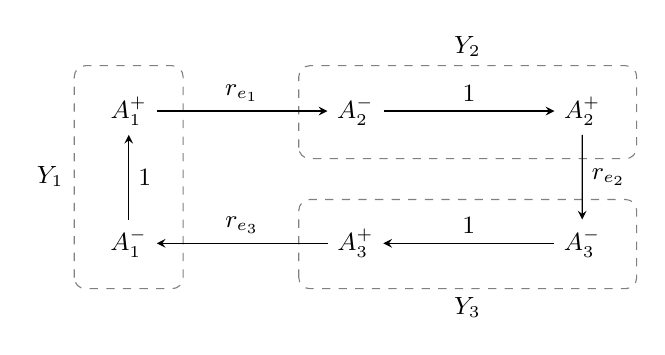
\begin{tikzpicture}[>=stealth,scale=.96,
   every node/.style={font=\small}]
  \draw[dashed,rounded corners,gray] (-.72,-.7) rectangle (.72,2.25);
  \draw[dashed,rounded corners,gray] (2.25,1.02) rectangle (6.72,2.25);
  \draw[dashed,rounded corners,gray] (2.25,-.7) rectangle (6.72,.48);
  \node at (-1.04,.78) {$Y_1$};
  \node at (4.48,2.5) {$Y_2$};
  \node at (4.48,-.95) {$Y_3$};
  \node (a) at (0,1.65) {$A_1^+$};
  \node (b) at (3,1.65) {$A_2^-$};
  \node (c) at (6,1.65) {$A_2^+$};
  \node (d) at (6,-.1) {$A_3^-$};
  \node (e) at (3,-.1) {$A_3^+$};
  \node (f) at (0,-.1) {$A_1^-$};
  \draw[->] (a) -- node[above] {$r_{e_1}$} (b);
  \draw[->] (b) -- node[above] {$1$} (c);
  \draw[->] (c) -- node[right] {$r_{e_2}$} (d);
  \draw[->] (d) -- node[above] {$1$} (e);
  \draw[->] (e) -- node[above] {$r_{e_3}$} (f);
  \draw[->] (f) -- node[right] {$1$} (a);
 \end{tikzpicture}
 \caption{A conductor cycle represented by birational maps between
 minimal strata.  Each dashed box groups two choices inside one dlt
 component; it does not depict geometric intersections.  The arrows
 are birational comparisons, labelled by their pullback multipliers.
 Their composition acts on $A_1^+$ with multiplier
 $r_{e_1}r_{e_2}r_{e_3}$.}
 \label{res:figure}
 \end{figure}

 Choose
 \begin{equation}\label{res:uniform-exponent}
  L=\operatorname{lcm}\{L(q,m):0\le q\le d-1\},
  \qquad a=mL,
 \end{equation}
 where $L(q,m)$ is given by Theorem~\ref{thm:characters}.
 Applying that theorem to \eqref{res:cycle} shows that the product
 of $r_e^L$ around every closed walk is one.  Consequently there
 are constants $c_i\in\C^*$ satisfying
 \begin{equation}\label{res:scales}
  c_i=c_jr_e^L\quad\text{for every oriented edge }e:i\to j.
 \end{equation}
 For completeness, choose a spanning tree in each connected
 component, set $c_i=1$ at one vertex, and determine the other
 constants along its tree paths.  Every additional edge is
 consistent because it closes a walk with product one.  A loop
 imposes precisely $r_e^L=1$, already proved.

 The forms $c_i\theta_i^{\otimes L}$ now have equal residues on
 every pair of conductor branches.  Regard their tuple as a
 rational $a$-canonical form $\sigma$ on $X$: it is an element
 of the product of the degree-$a$ canonical lines of the component
 function fields, a rank-one module over the total quotient ring
 $\prod_i\C(X_i)$.  At every normal
 codimension-one point, its divisor says that it generates the
 line corresponding to $aD$.  At each generic node, its branches
 are generators and have matching residues, so the local rule
 \eqref{res:node-generator} makes it a generator there as well;
 $a$ is even and $B$ avoids those points.

 We explain why this proves Cartierness, rather than only
 triviality after normalization.  Choose a big open immersion
 $j:U\hookrightarrow X$ containing all codimension-one points,
 such that $X$ is Gorenstein on $U$, $aB$ is Cartier on $U$, and
 the preceding local comparisons make $\sigma$ a generator of
 \[
  \mathcal L_{a,U}=\omega_U^{\otimes a}(aB|_U).
 \]
 The divisorial sheaf associated with $aD$ is its $S_2$ extension
 $\mathcal F_a=j_*\mathcal L_{a,U}$.  The generator identifies
 this sheaf with $j_*\OO_U=\OO_X$, the last equality following
 from $S_2$.  Hence $\mathcal F_a$ is invertible.  Equivalently,
 divide $\sigma$ by the $a$th power of a rational canonical
 form, chosen to generate at the generic nodes.  The ratio is
 an invertible element of the total quotient ring whose
 principal divisor is $-aD$ on $U$ and therefore on $X$.
 Thus $aD$ is principal Cartier.  Isolated vertices of the
 conductor graph cause no difficulty: their chosen forms
 already satisfy the required condition.

 Finally let the ground field $k$ be any algebraically closed field
 of characteristic zero.  All the data descend to an algebraically
 closed subfield $k_0\subset k$ of finite transcendence degree over
 $\Q$, including the normalization, conductor, a principal Cartier
 multiple of $D$, and a log resolution of the normalized pair.
 The field $k_0$ embeds in $\C$.  The hypotheses persist under these
 algebraically closed field extensions: $S_2$ and the smooth or
 nodal codimension-one charts are preserved, normalization and
 conductor commute with them, and the coefficients on the chosen
 log resolution test log canonicity after extension.  We therefore
 obtain the degree-$a$ conclusion over $\C$ with the same integer
 \eqref{res:uniform-exponent}.

 On a fixed big Gorenstein open over $k_0$, form $\mathcal F_a$ as
 above.  The open immersion is quasi-compact and separated, since
 $X$ is noetherian.  Flat base change for quasi-coherent sheaves
 therefore shows that this extension by $j_*$ commutes with field
 extension, so its pullback to $\C$ is trivial.  Invertibility
 descends faithfully flatly.  For the resulting line bundle,
 proper cohomology and field extension identify its space of
 global sections after extension with $H^0(X_{\C},\OO_{X_{\C}})
 =\C$.  Its one-dimensional space over $k_0$ therefore has a
 nonzero section whose evaluation becomes an isomorphism over
 $\C$ and hence is already an isomorphism over $k_0$.  Thus
 $\mathcal F_a\simeq\OO$ over $k_0$, and extending to $k$ proves
 the theorem.
\end{proof}
